\documentclass[12pt,letterpaper]{article}
\usepackage[body={18cm, 25cm}]{geometry}
\usepackage[spanish, activeacute]{babel}
\usepackage[utf8]{inputenc}
\decimalpoint
\usepackage{natbib}
\usepackage{lscape}
\usepackage{amsmath}
\usepackage{amsfonts}
\usepackage{amssymb}
\usepackage{graphicx}
\usepackage{geometry}
\usepackage{float}
%\usepackage{subfloat}
\usepackage{caption}
\usepackage{subcaption}
\usepackage{algpseudocode}
%\usepackage{subfig}%%Para incluir subgraficos
\usepackage{fancyhdr}%%Para incluir encabezado
\usepackage[pdftex, pdftitle={Rotación de Vectores}, pdfauthor={J. Vergara}, pdfsubject={Vectors}, pdfkeywords={vectores, rotación, mecánica del medio continuo}, pdfpagemode=UseOutlines,bookmarks,bookmarksopen,pdfstartview=FitH,colorlinks,linkcolor=blue, urlcolor=black, citecolor=blue]{hyperref}
\geometry{verbose,letterpaper,tmargin=3cm,bmargin=3cm,lmargin=3cm,rmargin=3cm}


\author{Juan Carlos Vergara Gallego - Grupo de Investigación en Mecánica Aplicada \\ Universidad EAFIT}
\title{\textbf{Rotación de Vectores, Caso $2D$ y $3D$}}

\usepackage{cleveref}
\begin{document}

\pagestyle{fancyplain}
\fancyhf{}
%\fancyheadoffset[LE,RO]{\marginparsep+\marginparwidth}
\headheight=20pt %para cambiar el tamaño del encabezado
\renewcommand{\headrulewidth}{0pt} %espesor del encabezado

\lhead %la "L" indica a la izquierda
{
\begin{minipage}{3cm}

\includegraphics[width=1.5 in]{img/logo.pdf}
\end{minipage}
}

\fancyfoot[c]{\thepage}

\maketitle


{\bf Palabras clave:} Vector, Rotación,Matriz de transformación\\\\

\abstract
%
El procedimiento para expresar un vector que se encuentra descrito en el sistema de referencia cartesiano $x-y-z$ en otro sistema de referencia cartesiano $x'-y'-z'$ es presentado. Como base del procedimiento se explica como se obtiene la matriz de transfomación. 
%
%En matemáticas las rotaciones son transformaciones lineales que conservan las normas en espacios vectoriales en los que se ha definido una operación de producto interior. La matriz de transformación tiene la propiedad de ser una matriz unitaria, es decir, es ortogonal y su determinante es 1. Sea un vector \scriptstyle \mathbf A expresado en un sistema de coordenadas cartesianas (x, y, z) con una base vectorial \mathcal{B} asociada definida por los versores \left( \mathbf i, \mathbf j,\mathbf k\, \right); esto es,
%
\section{Planteamiento del problema}
%
Lo que se pretende encontrar es una relación matemática que permita  expresar un vector  $\overset{\rightarrow}{V}$ que se encuentra descrito en el sistema de referencia cartesiano $x-y-z$ en otro sistema de referencia cartesiano $x'-y'-z'$. En las figuras \ref{planteamiento} y \ref{planteamiento3d} se presenta la descripción gráfica del problema para el caso bidimensional y el caso tridimensional respectivamente.  
%
\begin{figure}[H]
%	\centering
%	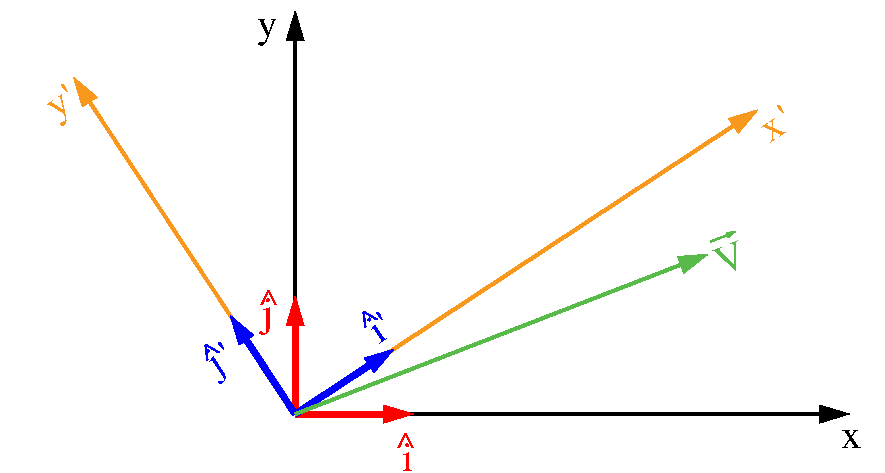
\includegraphics[width=15cm]{img/Planteamiento.pdf}
%	\caption{Ángulos entre los ejes de ambos sistemas de referencia.}
%	\label{planteamiento}
%	
	\centering
	\begin{subfigure}[l]{0.450\textwidth}
		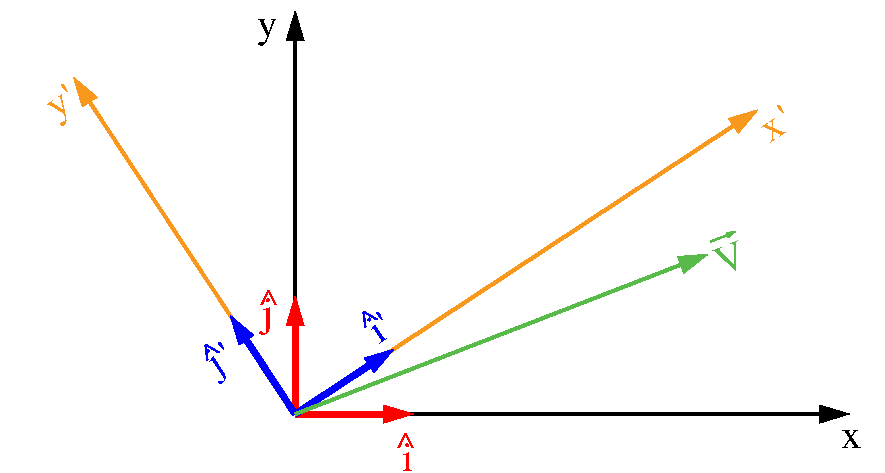
\includegraphics[width=\textwidth]{img/Planteamiento.pdf}
		\caption{Problema 2D.}
		\label{planteamiento}
	\end{subfigure}
	\hspace{.5 cm}
	%
	\begin{subfigure}[r]{0.450\textwidth}
		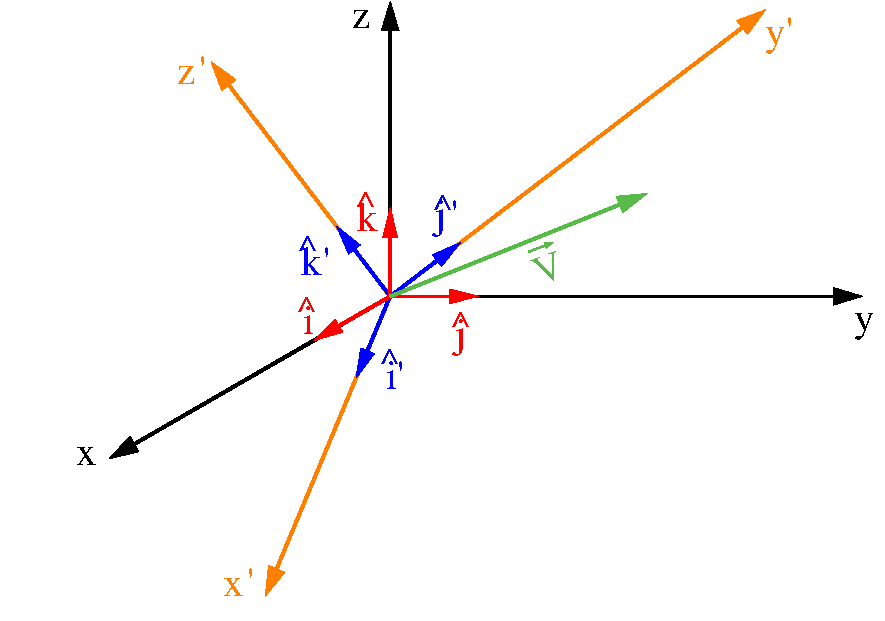
\includegraphics[width=\textwidth]{img/Planteamiento3D.pdf}
		\caption{Problema 3D.}
		\label{planteamiento3d}
	\end{subfigure}	
	\caption{}
\end{figure}
%
%
\section{Desarrollo del problema $2D$}
%
Para dar solución al problema basta conocer las componentes del vector en el sistema de referencia original $x-y$ y los cosenos directores  (cosenos de los ángulos) entre el sistema de referencia $x-y$ y el sistema de referencia $x'-y'$. En la figura \ref{direc2d} se muestran los ángulos entre el sistema de referencia $x-y$ y el sistema de referencia $x'-y'$ junto con los vectores unitarios de cada base ortonormal $\left( \hat{i}, \hat{j} \right)$ y $\left( \hat{i}', \hat{j}' \right)$.\\\\
%
%
\begin{figure}[H]
	\centering
	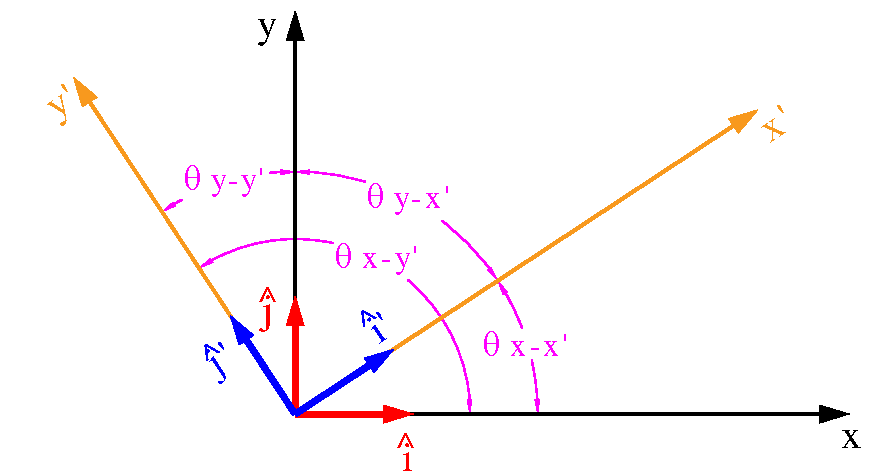
\includegraphics[width=15cm]{img/Directores2D.pdf}
	\caption{Ángulos entre los ejes de ambos sistemas de referencia.}
	\label{direc2d}
\end{figure}

Donde:
%
\begin{itemize}
	\item[$\rightarrow$] \begin{large}$\theta_{x-x'}$\end{large}: Ángulo entre el eje \begin{large}$x$\end{large} y el eje \begin{large}$x'$\end{large}.
	\item[$\rightarrow$] \begin{large}$\theta_{x-y'}$\end{large}: Ángulo entre el eje \begin{large}$x$\end{large} y el eje \begin{large}$y'$\end{large}.
	\item[$\rightarrow$] \begin{large}$\theta_{y-x'}$\end{large}: Ángulo entre el eje \begin{large}$y$\end{large} y el eje \begin{large}$x'$\end{large}.
	\item[$\rightarrow$] \begin{large}$\theta_{y-y'}$\end{large}: Ángulo entre el eje \begin{large}$y$\end{large} y el eje \begin{large}$y'$\end{large}.
	\item[$\rightarrow$] \begin{large}$\hat{i}$, $\hat{j}$\end{large}: Vectores unitarios bases del sistema de referencia \begin{large}$x-y$\end{large}.
	\item[$\rightarrow$] \begin{large}$\hat{i}'$, $\hat{j}'$\end{large}: Vectores unitarios bases del sistema de referencia \begin{large}$x'-y'$\end{large}.\\\\
\end{itemize}
%
%
El vector a transformar de sistema de referencia cartesiano lo denominaremos $\overset{\rightarrow}{V}$ en el sistema de referencia $x-y$ y $\overset{\rightarrow}{V'}$ en el sistema de referencia $x'-y'$. En las figuras \ref{vector1} y  \ref{vector2} se muestra cada vector en su base vectorial y en las  figuras \ref{vector1comp} y \ref{vector2comp} se presenta el vector a transformar junto con su proyección sobre cada uno de los ejes del sistema de referencia.\\\\
%
%
\begin{figure}[H]
	\centering
	\begin{subfigure}[l]{0.45\textwidth}
		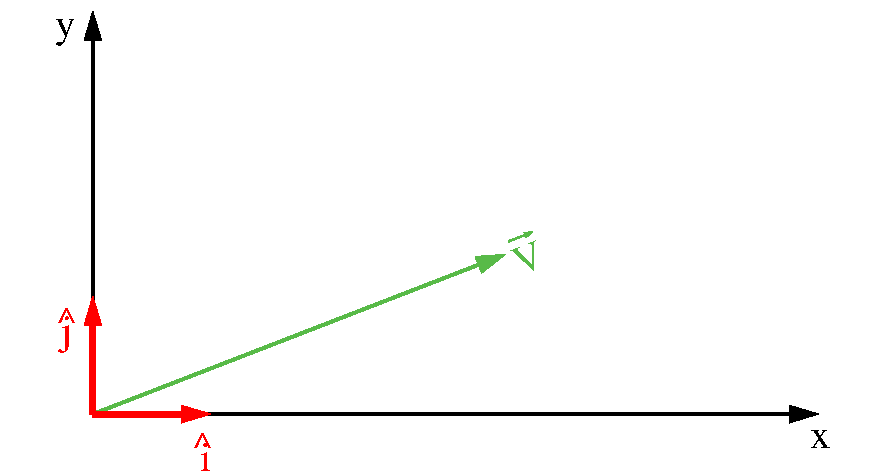
\includegraphics[width=\textwidth]{img/Vector1.pdf}
		\caption{Vector $\overset{\rightarrow}{V}$ en el sistema de referencia $x-y$.}
		\label{vector1}
	\end{subfigure}
	\hspace{.5 cm}
	%
	\begin{subfigure}[r]{0.45\textwidth}
		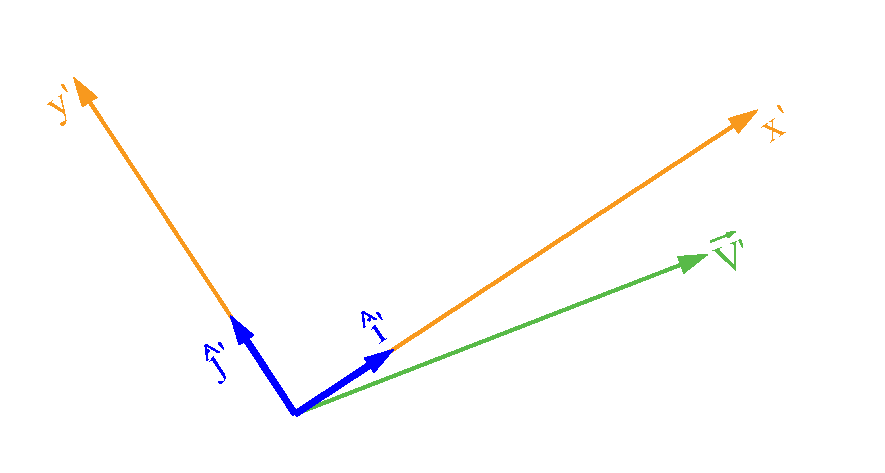
\includegraphics[width=\textwidth]{img/Vector2.pdf}
		\caption{Vector $\overset{\rightarrow}{V'}$ en el sistema de referencia $x'-y'$.}
		\label{vector2}
	\end{subfigure}	
	\caption{}
\end{figure}
%

%Adicionalmente, en la figuras \ref{vector1comp} y \ref{vector2comp} se presenta el vector a transformar junto con su proyección sobre cada uno de los ejes del sistema de referencia.\\\\

\begin{figure}[H]
	\centering
	\begin{subfigure}[l]{0.450\textwidth}
		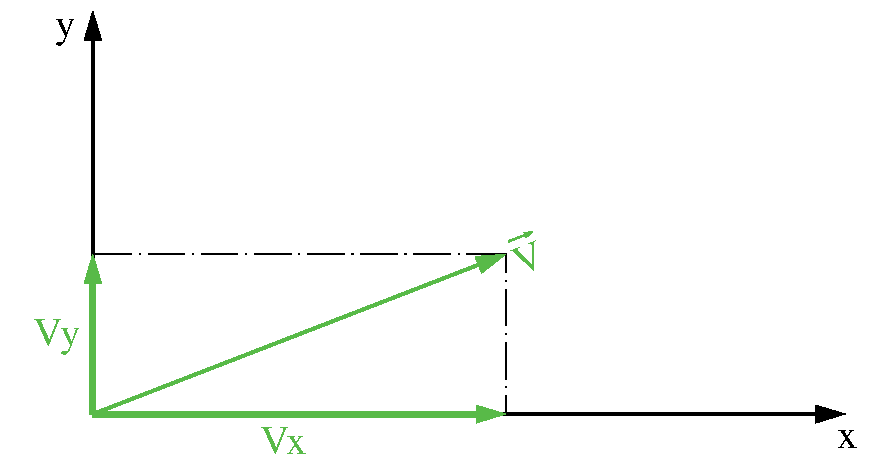
\includegraphics[width=\textwidth]{img/Vector1Componentes.pdf}
		\caption{Vector $\overset{\rightarrow}{V}$ en el sistema de referencia $x-y$.}
		\label{vector1comp}
	\end{subfigure}
	\hspace{.5 cm}
	%
	\begin{subfigure}[r]{0.450\textwidth}
		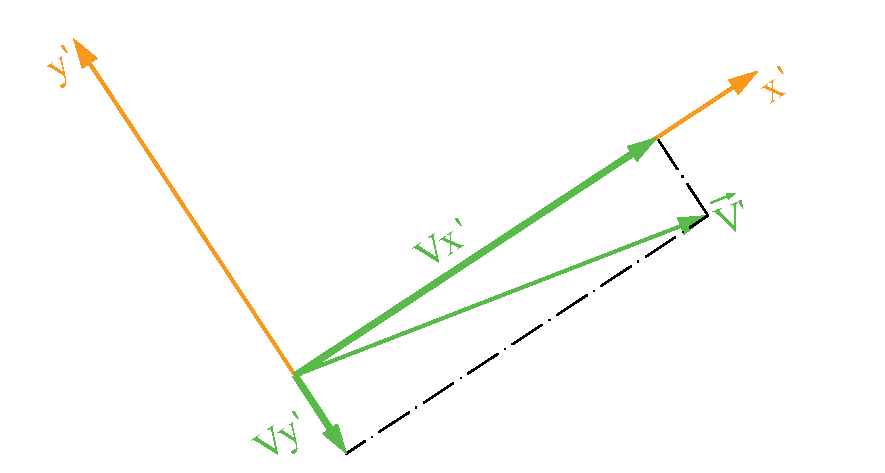
\includegraphics[width=\textwidth]{img/Vector2Componentes.pdf}
		\caption{Vector $\overset{\rightarrow}{V'}$ en el sistema de referencia $x'-y'$.}
		\label{vector2comp}
	\end{subfigure}	
	\caption{}
\end{figure}
%
%
El vector $\overset{\rightarrow}{V}$ y el vector $\overset{\rightarrow}{V'}$ son equivalentes, (iguales) en ambos sistemas de referencia, debido a que la magnitud y significado físico no varía por tener diferente sistema de referencia. Lo único diferente entre estos es la forma de representarlos en términos de sus componentes. Por esta razón se puede decir que:
%
\begin{align}
	\overset{\rightarrow}{V} = \overset{\rightarrow}{V'}
	\label{uno}
\end{align}
%
Si se escribe el vector $\overset{\rightarrow}{V}$  y  $\overset{\rightarrow}{V'}$ y en términos de sus compenentes escalares (figura \ref{vector1comp} y \ref{vector2comp}), se tiene: 

%Es posible expresar el vector en cada base ortogonal a partir de sus componentes escalares (figura \ref{vector1comp} y \ref{vector2comp}), como se muestra en las ecuaciones \ref{dos} y \ref{tres}.
%
\begin{align}
	\overset{\rightarrow}{V} = V_x \hat{i} + V_y \hat{j} \label{dos}  \\
	\overset{\rightarrow}{V'} = V_{x'} \hat{i'} + V_{y'} \hat{j'} \label{tres}
\end{align}\

Expresando el vector unitario $\hat{i}$ y $\hat{j}$ en términos de los vectores unitarios $\hat{i}'$ y $\hat{j}'$, se obtiene que la ecuación \ref{dos} podría escribirse como: 
%
%\begin{align}
%	\hat{i} = \hat{i}' \cos \theta_{x-x'} +  \hat{j}' \cos \theta_{x-y'} \label{cuatro}\\
%	\hat{j} = \hat{i}' \cos \theta_{y-x'} +  \hat{j}' \cos \theta_{y-y'} \label{cinco}
%\end{align}
%%
%Reemplazando las ecuaciones \ref{cuatro} y \ref{cinco} en la ecuación \ref{dos}:

\begin{align*}
	\overset{\rightarrow}{V} = V_x \left( \hat{i}' \cos \theta_{x-x'} + \hat{j}' \cos \theta_{x-y'} \right) + V_y \left( \hat{i}' \cos \theta_{y-x'} + \hat{j}' \cos \theta_{y-y'} \right)
\end{align*} \

Reorganizando los términos:
%
\begin{align}
	\overset{\rightarrow}{V} = \left( V_x \cos \theta_{x-x'} + V_y \cos \theta_{y-x'} \right) \hat{i}'+ \left( V_x \cos \theta_{x-y'} + V_y \cos \theta_{y-y'} \right) \hat{j}' \label{seis}
\end{align}
%
Reemplazando las ecuaciones \ref{seis} y \ref{tres} en la ecuación \ref{uno}:
%
\begin{align}
	\left( V_x \cos \theta_{x-x'} + V_y \cos \theta_{y-x'} \right) \hat{i}'+ \left( V_x \cos \theta_{x-y'} + V_y \cos \theta_{y-y'} \right) \hat{j}' = V_{x'} \hat{i}' + V_{y'} \hat{j}' \label{siete}
\end{align}
%
Como puede verse ambos lados de la ecuación \ref{siete} contiene términos que dependen de $\hat{i}'$
y $\hat{j}'$. Igualando los términos que dependen de $\hat{i}'$ y los que dependen de $\hat{j}'$, se obtiene el sistema formado por las ecuaciones \ref{ocho} y \ref{nueve} :
%
\begin{align}
	V_x \cos \theta_{x-x'} + V_y \cos \theta_{y-x'} = V_{x'} \label{ocho}\\
	V_x \cos \theta_{x-y'} + V_y \cos \theta_{y-y'} = V_{y'} \label{nueve}
\end{align}
%
%Las ecuaciones \ref{ocho} y \ref{nueve} las expresamos matricialmente:
Expresando matricialmente: 
%
\begin{eqnarray}
		\left[ \begin{array}{c} V_{x'} \\
		V_{y'} \end{array} \right] = 
		\left[ \begin{array}{cc}
		\cos \theta_{x-x'} & \cos \theta_{y-x'} \\  
		\cos \theta_{x-y'} & \cos \theta_{y-y'}
		\end{array}  \right] 
		\left[ \begin{array}{c} V_{x} \\
		V_{y} \end{array} \right]
		\label{diez}
\end{eqnarray}
%
En la ecuación \ref{diez} se identifican los siguientes elementos:
%
\begin{align*}
	\left[ \begin{array}{c}
		V_x \\
		V_y	
	\end{array} \right]: \textup{Componentes del vector $\overset{\rightarrow}{V}$ en el sistema de referencia $x-y$} 
\end{align*}
%
\begin{align*}
	\left[ \begin{array}{c}
		V_{x'} \\
		V_{y'}	
	\end{array} \right]: \textup{Componentes del vector $\overset{\rightarrow}{V'}$ en el sistema de referencia $x'-y'$} 
\end{align*}
%
\begin{align}
	\left[ T \right] = \left[ \begin{array}{cc}
		\cos \theta_{x-x'} & \cos \theta_{y-x'} \\
		\cos \theta_{x-y'} & \cos \theta_{y-y'}	
	\end{array} \right] \label{once}
\end{align}
%
La  ecuación \ref{once} corresponde a la matriz de transformación, la cual permite representar entidades físico-matemáticas, descritas en el sistema de referencia $x-y$, en el sistema de referencia $x'-y'$.\\\\

Por otra parte, si lo que se conoce es el vector en el sistema de referencia $x'-y'$ y se quire  expresar en el sistema de referencia $x-y$, solo es necesario realizar manipulaciones matemáticas simples sobre la ecuación \ref{diez}.\\
%
Reescribiendo la ecuación \ref{diez}:
%
\begin{align*}
	\left[ V' \right] = \left[ T \right] \left[ V \right]
\end{align*}
%
Premultiplicando la ecuación \ref{diez} por la inversa de la matriz de transformación:
%
\begin{align*}
	\left[ T \right]^{-1} \left[ V' \right] = \left[ T \right]^{-1} \left[ T \right] \left[ V \right]
\end{align*}
%
Ya que $\left[ T \right]$ es una matriz de transformación entre dos sistemas de referencia ortogonales, se tiene que $\left[ T \right]^{-1} = \left[ T \right]^T$. Además, se tiene que $\left[ T \right] \left[ T \right]^T = \left[ I \right]$ y que $\left[ I \right] \left[ V \right] = \left[ V \right]$.
%
\begin{align}
	\left[ V \right] = \left[ T \right]^T \left[ V' \right] \label{doce}
\end{align}
%
La ecuación \ref{doce} permite expresar el vector $\overset{\rightarrow}{V'}$ del sistema de referencia $x'-y'$ en el sistema de referencia $x-y$.\\\\
%
¿Cómo leer y/o hallar la matriz de transformación $\left[ T \right]$?.\\\\
Lectura de columnas:
%
\begin{itemize}
	\item Columna 1: $ \left[ \begin{array}{c}
		\cos \theta_{x-x'} \\	 \cos \theta_{x-y'}
	\end{array} \right]$, vector que contiene los cosenos de los ángulos entre el eje $x$ del sistema de referencia original y los ejes $x'$ y $y'$ (ver figura \ref{planteamiento}).
	\item Columna 2: $ \left[ \begin{array}{c}
		\cos \theta_{y-x'} \\	 \cos \theta_{y-y'}
	\end{array} \right]$, vector que contiene los cosenos de los ángulos entre el eje $y$ del sistema de referencia original y los ejes $x'$ y $y'$ (ver figura \ref{planteamiento}).
\end{itemize}
%
Lectura de filas:
%
\begin{itemize}
	\item Fila 1: $ \left[ \begin{array}{cc}
		\cos \theta_{x-x'} &	 \cos \theta_{y-x'}
	\end{array} \right]$, vector que contiene los cosenos de los ángulos entre los ejes $x$ y $x'$ y entre los ejes $y$ y $x'$ (ver figura \ref{planteamiento}).
	\item Fila 2: $ \left[ \begin{array}{cc}
		\cos \theta_{x-y'} &	 \cos \theta_{y-y'}
	\end{array} \right]$, vector que contiene los cosenos de los ángulos entre los ejes $x$ y $y'$ y entre los ejes $y$ y $y'$ (ver figura \ref{planteamiento}).
\end{itemize}
%
{\bf Nota importante: } Se utiliza la función trigonométrica {\it{Coseno}} pues esta es una función par y por ende no importa el signo del ángulo entre los ejes.\\
$\cos \left( -\theta \right) = \cos \left( \theta \right)$.\\\\


\section{Desarrollo del problema $3D$}
%
El caso tridimensional $(3D)$ no es nada más que una extensión del caso bidimensional $(2D)$, por lo cual en este documento solo se muestra que se le debe adicionar a las ecuaciones descritas en el caso $(2D)$. 

En la figura \ref{directores} se presenta el vector a transformar, denominado $\overset{\rightarrow}{V}$ en el sistema de referencia $x-y-z$ y $\overset{\rightarrow}{V'}$ en el sistema de referencia $x'-y'-z'$. En las figuras \ref{vector13d} y \ref{vector23d} se presenta dicho vector en cada sistema de referencia y en las figuras \ref{vector1comp3d} y \ref{vector2comp3d} se presenta el vector junto con sus proyecciones escalares.\\\\

\begin{figure}[H]
	\centering
	\begin{subfigure}[l]{0.450\textwidth}
		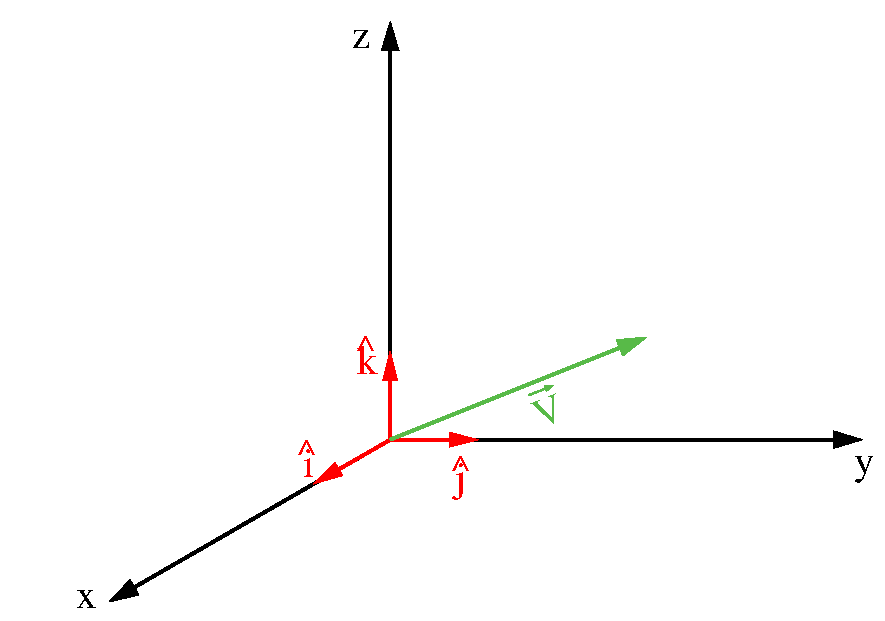
\includegraphics[width=\textwidth]{img/Vector13D.pdf}
		\caption{Vector $\overset{\rightarrow}{V}$ en el sistema de referencia $x-y$.}
		\label{vector13d}
	\end{subfigure}
	\hspace{.5 cm}
	%
	\begin{subfigure}[r]{0.450\textwidth}
		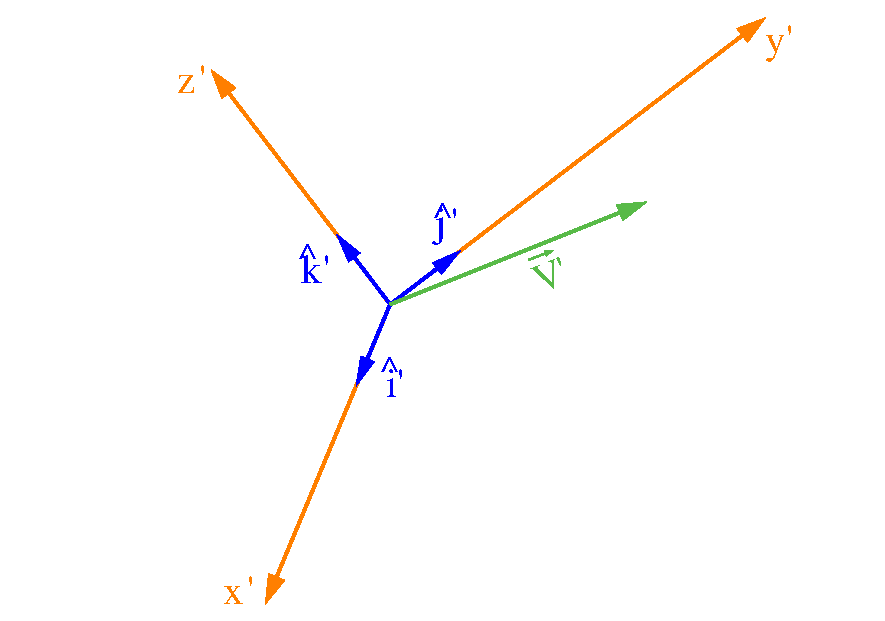
\includegraphics[width=\textwidth]{img/Vector23D.pdf}
		\caption{Vector $\overset{\rightarrow}{V'}$ en el sistema de referencia $x'-y'$.}
		\label{vector23d}
	\end{subfigure}	
%
	\begin{subfigure}[l]{0.450\textwidth}
		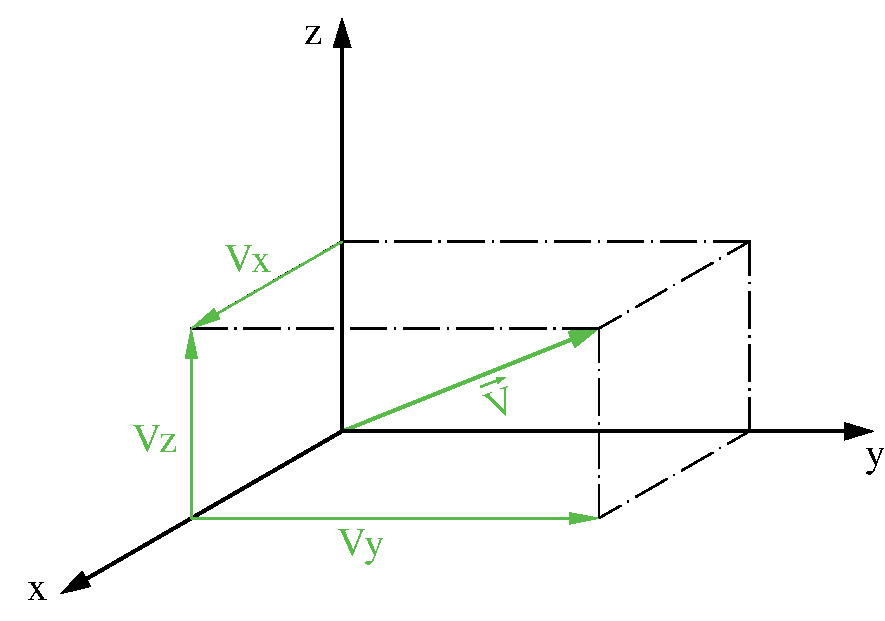
\includegraphics[width=\textwidth]{img/Vector1Componentes3D.pdf}
		\caption{Vector $\overset{\rightarrow}{V}$ en el sistema de referencia $x-y$.}
		\label{vector1comp3d}
	\end{subfigure}
	\hspace{.5 cm}
	%
	\begin{subfigure}[r]{0.450\textwidth}
		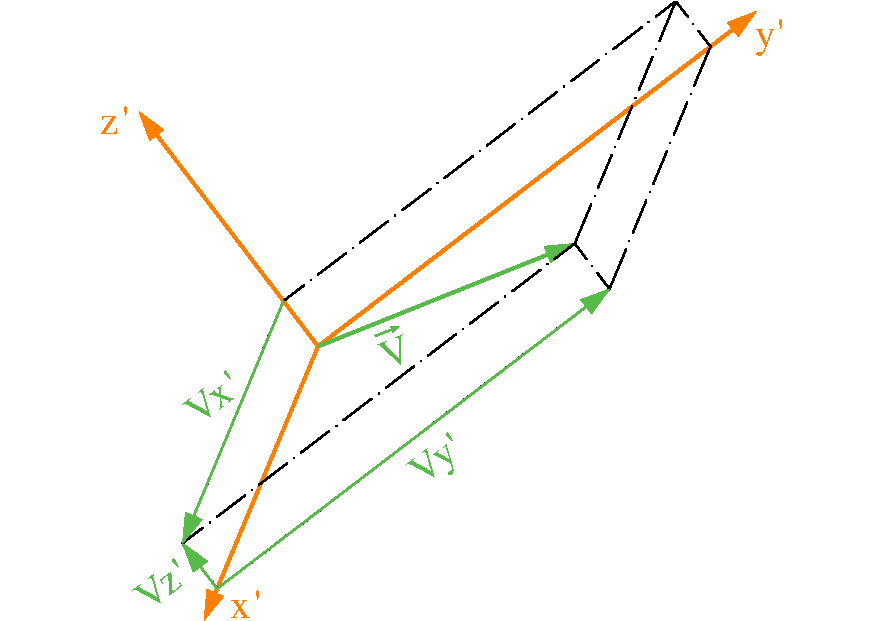
\includegraphics[width=\textwidth]{img/Vector2Componentes3D.pdf}
		\caption{Vector $\overset{\rightarrow}{V'}$ en el sistema de referencia $x'-y'$.}
		\label{vector2comp3d}
	\end{subfigure}	
	\caption{}
	\label{directores}
\end{figure}
%
%
%
%
%
En la figura \ref{directorestodos} se presentan los ángulos entre los ejes del sistema de referencia $x-y-z$ y el sistema de referencia $x'-y'-z'$ , junto con los vectores unitarios de cada base ortogonal $\left( \hat{i}, \hat{j}, \hat{k} \right)$ y $\left( \hat{i}', \hat{j}', \hat{k}' \right)$.\\\\

\begin{figure}[H]
	\centering
	\begin{subfigure}[l]{0.450\textwidth}
		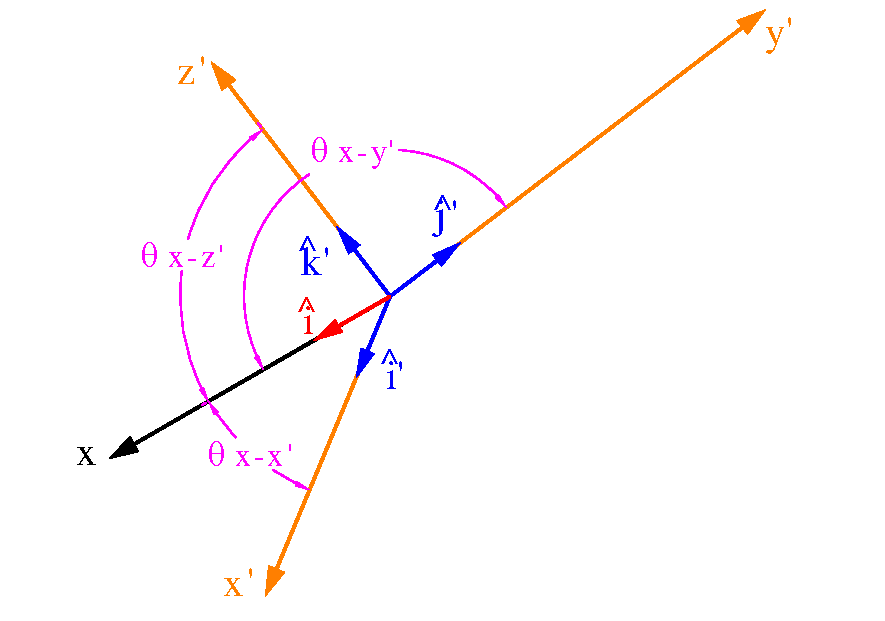
\includegraphics[width=\textwidth]{img/CosenosX3D.pdf}
		\caption{Vector $\overset{\rightarrow}{V}$ en el sistema de referencia $x-y$.}
		\label{cosx3d}
	\end{subfigure}
	\hspace{.5 cm}
	%
	\begin{subfigure}[r]{0.450\textwidth}
		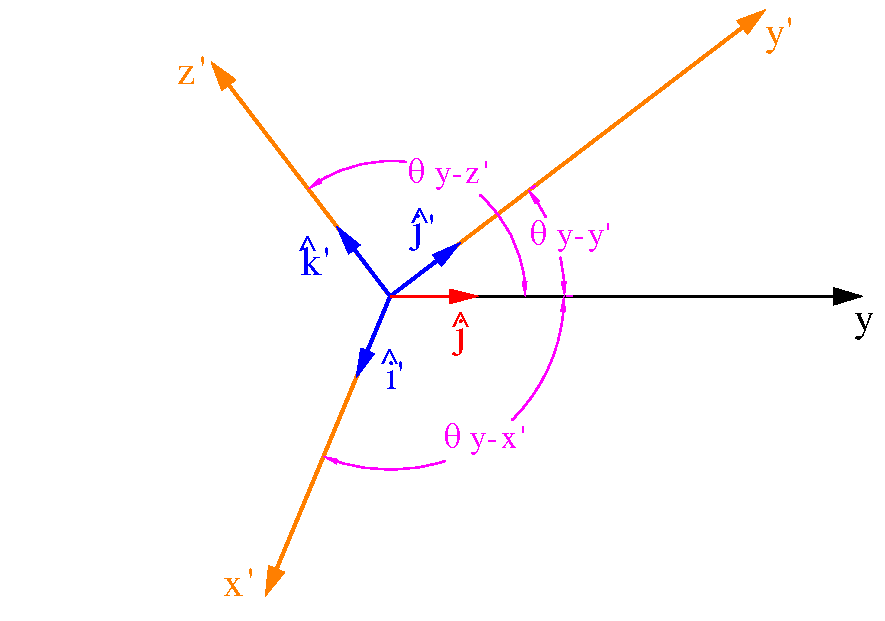
\includegraphics[width=\textwidth]{img/CosenosY3D.pdf}
		\caption{Vector $\overset{\rightarrow}{V'}$ en el sistema de referencia $x'-y'$.}
		\label{cosy3d}
	\end{subfigure}
	%
	\begin{subfigure}[r]{0.450\textwidth}
		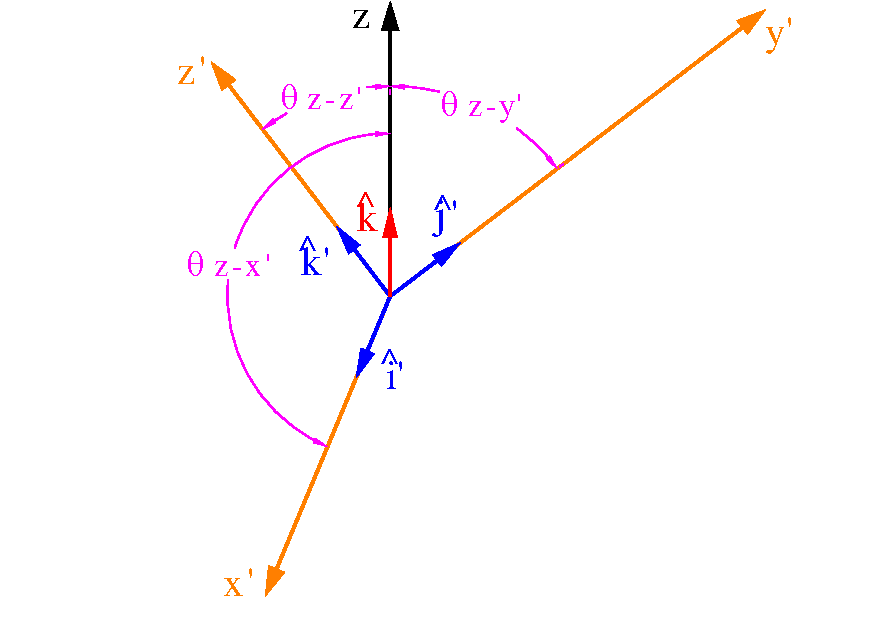
\includegraphics[width=\textwidth]{img/CosenosZ3D.pdf}
		\caption{Vector $\overset{\rightarrow}{V'}$ en el sistema de referencia $x'-y'$.}
		\label{cosz3d}
	\end{subfigure}	
	\caption{}
	\label{directorestodos}
\end{figure}

%
%
%
%
%

%
\begin{itemize}
	\item \begin{large}$\theta_{x-x'}$\end{large}: Ángulo entre el eje $x$ y el eje $x'$
	\item \begin{large}$\theta_{x-y'}$\end{large}: Ángulo entre el eje $x$ y el eje $y'$
	\item \begin{large}$\theta_{x-z'}$\end{large}: Ángulo entre el eje $x$ y el eje $z'$
	\item \begin{large}$\theta_{y-x'}$\end{large}: Ángulo entre el eje $y$ y el eje $x'$
	\item \begin{large}$\theta_{y-y'}$\end{large}: Ángulo entre el eje $y$ y el eje $y'$
	\item \begin{large}$\theta_{y-z'}$\end{large}: Ángulo entre el eje $y$ y el eje $z'$
	\item \begin{large}$\theta_{z-x'}$\end{large}: Ángulo entre el eje $z$ y el eje $x'$
	\item \begin{large}$\theta_{z-y'}$\end{large}: Ángulo entre el eje $z$ y el eje $y'$
	\item \begin{large}$\theta_{z-z'}$\end{large}: Ángulo entre el eje $z$ y el eje $z'$
	\item \begin{large}$\hat{i}$, $\hat{j}$, $\hat{k}$\end{large}: Vectores unitarios bases del sistema de referencia $x-y-z$.
	\item \begin{large}$\hat{i}'$, $\hat{j}'$, $\hat{k}'$\end{large}: Vectores unitarios bases del sistema de referencia $x'-y'-z'$.
\end{itemize}
%
Por similitud a la ecuación \ref{diez} del caso bidimensional, se tiene: 
%
\begin{eqnarray}
		\left[ \begin{array}{c} V_{x'} \\
		V_{y'} \\ V_{z'} \end{array} \right] = 
		\left[ \begin{array}{ccc}
		\cos \theta_{x-x'} & \cos \theta_{y-x'} & \cos \theta_{z-x'} \\  
		\cos \theta_{x-y'} & \cos \theta_{y-y'} & \cos \theta_{z-y'} \\
		\cos \theta_{x-z'} & \cos \theta_{y-z'} & \cos \theta_{z-z'}
		\end{array}  \right] 
		\left[ \begin{array}{c} V_{x} \\
		V_{y} \\ V_{z} \end{array} \right]
		\label{trece}
\end{eqnarray}
%
Donde:
%
\begin{align}
	\left[ T \right] = \left[ \begin{array}{ccc}
		\cos \theta_{x-x'} & \cos \theta_{y-x'} & \cos \theta_{z-x'} \\  
		\cos \theta_{x-y'} & \cos \theta_{y-y'} & \cos \theta_{z-y'} \\
		\cos \theta_{x-z'} & \cos \theta_{y-z'} & \cos \theta_{z-z'}
		\end{array}  \right] \label{catorce}
\end{align}
%
El significado de las columnas y filas de la matriz de transformación $\left[ T \right]$ de la ecuación \ref{catorce} es el mismo al que se le dio para el caso de la matriz de transformación presentada en la ecuación \ref{once}.\\\\
%
Reescribiendo la ecuación \ref{trece} en forma compacta y la ecuación de transformación de $x'-y'-z'$ a $x-y-z$.
%
\begin{align*}
	\left[ V' \right] = \left[ T \right] \left[ V \right] \\
	\left[ V \right] = \left[ T \right]^T \left[ V' \right]
\end{align*}
%
%
\end{document}